\section{Experiments}
\label{sec:experiments}

\subsection{Experimental Setup}

\textbf{Evaluation and training.}\quad
We evaluate on $\tau^2$-Bench~\citep{tau2}, BFCL-v4 (multiturn)~\citep{bfcl},
ACEBench-Agent~\citep{acebench}, and AppWorld~\citep{appworld}.
The first three benchmarks use 1:1 public/private splits; AppWorld uses its
train split for public evaluation and test-normal split for private evaluation.
Public evaluation informs environment evolution and checkpoint
selection, while private evaluation is withheld from the evolution process and used
for final performance comparisons. Target models train with GRPO~\citep{grpo}.
Benchmark protocols, training configurations, and implementation versions are
given in Appendix~\ref{app:versions}.

\textbf{Implementation and baselines.}\quad
Our target models are Qwen3-4B-Instruct-2507 and Qwen3-8B~\citep{qwen3}, with
reasoning enabled for the latter.
Our data researcher agent, $\operatorname{DataResearcher}$, is instantiated
with Codex powered by GPT-6 Astra. We grant the agent access to the GPT-5.5 API
and 4 A100 GPUs during evolution. We compare against three baselines:
vanilla Codex as an autonomous data researcher (\texttt{Codex-Vanilla});
Codex with an example code repository provided (\texttt{Codex-E}); and
training on a fixed environment set generated by $\operatorname{DataResearcher}$
without revision (\texttt{Fixed-Env}). All researcher agents in these baselines
are powered by GPT-6 Astra.

\subsection{Main Results}
\label{sec:mainresults}

\suppressfloats[t] % Keep the results floats from floating above the setup.
\begin{table}[t]
\centering
\caption{Test performance (\%) at checkpoints selected on the public validation set. Green values show $\Delta$ from None (pp); Avg. averages all four benchmarks. Indented rows enable only the named component: BM, traceable behavioral map; CR, target-conditioned context refinement; EC, iterative environment construction. Dashes indicate unreported results.}
\label{tab:mainresults}
\begingroup
\small
\setlength{\tabcolsep}{4pt}
\setlength{\fboxsep}{1pt}
\renewcommand{\arraystretch}{1.0}
\setlength{\aboverulesep}{1.5pt}
\setlength{\belowrulesep}{1.5pt}
\definecolor{modelband}{HTML}{E7F6FD}
\definecolor{tablegain}{HTML}{218C4E}
\newcommand{\tabledelta}[2]{\mbox{#1\,{\scriptsize\textcolor{tablegain}{\textbf{#2}}}}}
\begin{tabular}{@{}m{.20\linewidth}@{}|@{}>{\centering\arraybackslash}m{.16\linewidth}@{}>{\centering\arraybackslash}m{.165\linewidth}@{}>{\centering\arraybackslash}m{.185\linewidth}@{}>{\centering\arraybackslash}m{.16\linewidth}@{}|@{}>{\centering\arraybackslash}m{\dimexpr.13\linewidth-2\arrayrulewidth\relax}@{}}
\toprule
\textbf{Method} & \textbf{$\tau^2$-Bench} & \textbf{BFCL-v4} &
\textbf{ACEBench-Agent} & \textbf{AppWorld} & \textbf{Avg.} \\
\midrule
\multicolumn{6}{@{}c@{}}{\colorbox{modelband}{\makebox[\dimexpr\linewidth-2\fboxsep\relax][c]{\strut\textit{\normalsize Qwen3-4B-Instruct-2507}}}} \\
\addlinespace[1pt]
None & 31.89 & 25.42 & 41.11 & 8.93 & 26.84 \\
\texttt{Codex-Vanilla} & \pending & \pending & \pending & \pending & \pending \\
\texttt{Codex-E} & \pending & \pending & \pending & \pending & \pending \\
\texttt{Fixed-Env} & \pending & \pending & \pending & \pending & \pending \\
\midrule
\method{} & \tabledelta{\textbf{39.33}}{+7.43} & \tabledelta{\textbf{42.08}}{+16.67} & \tabledelta{\textbf{52.22}}{+11.11} & \tabledelta{\textbf{22.22}}{+13.29} & \tabledelta{\textbf{38.96}}{+12.13} \\
\hspace{1em}$\hookrightarrow$\; BM-only & \pending & \pending & \pending & \pending & \pending \\
\hspace{1em}$\hookrightarrow$\; CR-only & \pending & \pending & \pending & \pending & \pending \\
\hspace{1em}$\hookrightarrow$\; EC-only & \pending & \pending & \pending & \pending & \pending \\
\addlinespace[3pt]
\multicolumn{6}{@{}c@{}}{\colorbox{modelband}{\makebox[\dimexpr\linewidth-2\fboxsep\relax][c]{\strut\textit{\normalsize Qwen3-8B (reasoning enabled)}}}} \\
\addlinespace[1pt]
None & 28.54 & 44.42 & 43.89 & \pending & \pending \\
\texttt{Codex-Vanilla} & \pending & \pending & \pending & \pending & \pending \\
\texttt{Codex-E} & \pending & \pending & \pending & \pending & \pending \\
\texttt{Fixed-Env} & \pending & \pending & \pending & \pending & \pending \\
\midrule
\method{} & \pending & \pending & \pending & \pending & \pending \\
\hspace{1em}$\hookrightarrow$\; BM-only & \pending & \pending & \pending & \pending & \pending \\
\hspace{1em}$\hookrightarrow$\; CR-only & \pending & \pending & \pending & \pending & \pending \\
\hspace{1em}$\hookrightarrow$\; EC-only & \pending & \pending & \pending & \pending & \pending \\
\bottomrule
\end{tabular}
\endgroup
\end{table}


\begin{figure}[t]
\centering
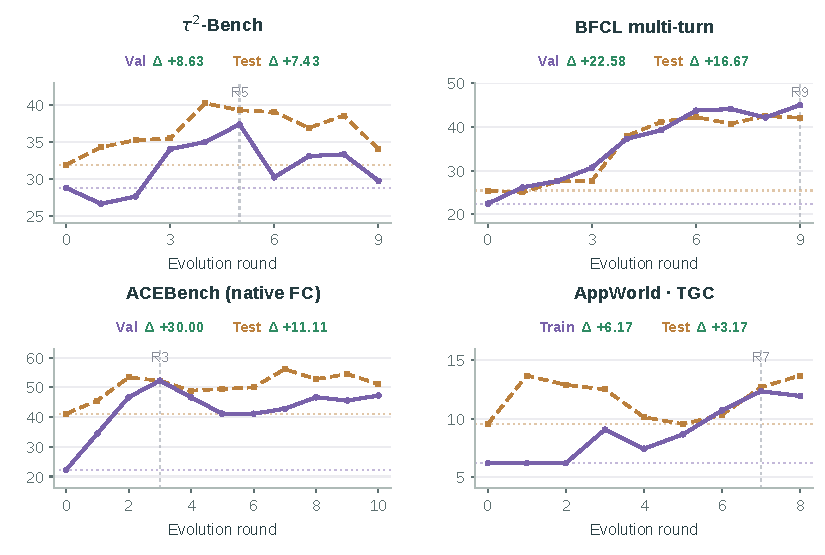
\includegraphics[width=\linewidth]{figures/evolution.pdf}
\caption{Public- and private-evaluation performance across environment-evolution rounds on four benchmarks, with Codex public-evaluation curves on $\tau^2$ and BFCL.}
\label{fig:evolution}
\end{figure}

\textbf{Strong coding agents struggle with continual data evolution.}\quad
Despite pairing GPT-6 Astra with the Codex harness, \texttt{Codex-Vanilla}
shows early gains followed by saturation or regression
(Figure~\ref{fig:evolution}). On BFCL, public performance peaks at 30.00\%
in R3 and falls to 25.42\% by R10.
On $\tau^2$, it finishes at 21.58\%, below its 27.10\% starting score.

A plausible bottleneck is maintaining the learning value of generated
environments as the target model changes. This requires updating training
targets from behavioral feedback and faithfully implementing the corresponding
mechanisms, the challenges identified in Section~\ref{sec:evidencegaps}.
Incomplete implementations or poorly updated targets may instead produce
executable environments that offer little additional learning signal.

\textbf{Substantial gains across four benchmarks.}\quad
\method{} improves 4B public-evaluation performance by $+8.63$, $+22.58$,
$+30.00$, and $+26.75$ percentage points over the base model on $\tau^2$-Bench,
BFCL-v4 (multiturn), ACEBench-Agent, and AppWorld, respectively. These results
use the earliest public maximum within the displayed rounds. The contrast is
clearest on BFCL: \method{} reaches 45.00\% in R9, well beyond
\texttt{Codex-Vanilla}'s 30.00\% peak in R3. On both benchmarks with baseline
curves, \method{} maintains higher scores throughout the shared R3--R9 rounds.
All four displayed endpoints remain above their starting scores.
Table~\ref{tab:mainresults} reports test performance at the validation-selected
checkpoints.

\subsection{Behavioral Coverage and Report Compactness}
\label{sec:analysiscoverage}

\begin{figure}[ht]
\centering
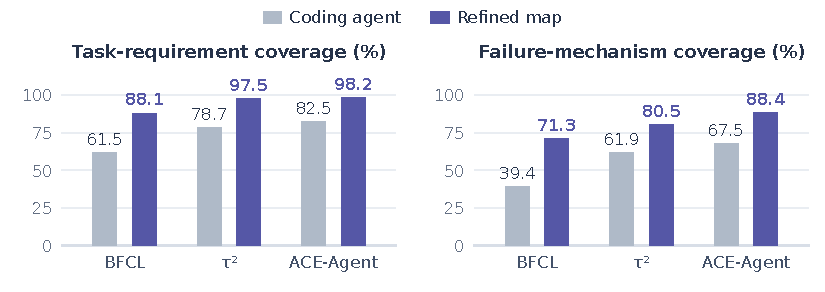
\includegraphics[width=\linewidth]{figures/analysis_coverage.pdf}
\caption{Task and failure coverage of the coding-agent reports and refined map
under the final paired evaluation. Report lengths and historical grades are
retained in Appendix~\ref{app:analysiscoverage}.}
\label{fig:analysiscoverage}
\end{figure}


We now test whether a structured analysis process reduces the information loss
identified in Section~\ref{sec:coveragegap}. On the same 1,692 frozen initial
Qwen3-8B public-eval trajectories, we compare the fixed coding-agent reports
(Astra/high) with a standalone, coverage-checked refinement of the behavioral
map (GPT-5.5/high). The refinement analyzes complete task evidence, consolidates
shared mechanisms, and checks the compact report for omitted conditions. It
receives neither the reference labels nor the coding agent's report prose.
We extend the same protocol to 243 initial public-eval trajectories of
Qwen3-4B-Instruct-2507 on AppWorld.

\textbf{Measure retained meaning, not compression alone.}\quad
Frozen, source-grounded reference units describe task requirements and failure
mechanisms. An LLM judge scores anonymized report pairs as full, partial,
missing, or contradicted. Only full preservation of the mechanism and its
consequential scope or dependency receives credit. We average units within
each task and then tasks within each corpus; word count separately measures
compactness. References are generated before seeing candidate reports, not
inferred from either method's preferred categories. Appendix~\ref{app:analysiscoverage}
gives the protocol, grading variability, costs, and spot audit.

\textbf{Higher coverage in shorter reports.}\quad
The refined map reaches 88.1--99.5\% task-requirement coverage and 71.3--88.4\%
failure-mechanism coverage, while using 12--29\% fewer words
(Figure~\ref{fig:analysiscoverage}a). It exceeds the paired
grades of the coding-agent reports on all four corpora; the ordering
also holds under subset--family-balanced aggregation. A concrete ACE example
shows why this is more than naming more error types: an inbox-cleanup timeout
label omits the user-authorization--deletion--retry dependency, which the
refined report preserves. Both graders support partial versus full coverage
for that example. Not every case improves; partially preserved mechanisms and
other collapsed distinctions are documented in Appendix~\ref{app:analysiscoverage}.

These development-set results support more comprehensive, compact behavioral
analysis in this setting. They do not isolate the hierarchy from the added
coverage checks, match backbones or computation, or establish downstream RL
gains. The diagnostic is separate from the historical 4B training runs.

\subsection{Training Signal across Evolution}
\label{sec:analysissignal}

We audit the saved RL reward groups from the original 4B experiments and
\texttt{Codex-Vanilla}. A task provides within-group reward signal when its
eight valid rollouts receive nonconstant rewards; we report the fraction of
such tasks among complete, valid groups in each round
(Figure~\ref{fig:researchdiagnostics}b). This measures the relative reward
contrast used by GRPO, retaining partial-credit rewards and excluding
incomplete groups rather than treating them as failures.

\textbf{Training success can exhaust the learning signal.}\quad
On $\tau^2$, every \texttt{Codex-Vanilla} task in R9 and R10 receives eight
rewards of one, leaving no within-group reward contrast. On BFCL, only
2 of 52 tasks retain reward variation in each of these rounds.
In comparison, \method{} retains signal on 70.5\% of valid $\tau^2$ tasks
and 35.5\% of BFCL tasks in its final recorded round, R9.
These observations motivate linking generated tasks to their actual training
outcomes so the researcher can detect reward saturation and refresh its
targets. They do not isolate the causal effect of context refinement.

\subsection{Environment Implementation Quality}
\label{sec:analysisenvironment}

\todo{Audit 20 sampled environments per benchmark, with eight rollouts each,
using an independent LLM judge to flag implementation, interaction, and verifier
defects. Replace the illustrative values in Figure~\ref{fig:researchdiagnostics}c
with measured environment-level audit pass rates (no defects flagged in the
inspected rollouts).}


\subsection{Remaining Controls and Uncertainty}

\textbf{Controls still required.}\quad
The available baseline records cover \texttt{Codex-Vanilla}; \texttt{Codex-E} and \texttt{Fixed-Env} comparisons are not yet reported. The offline diagnostic measures report quality, not a budget-matched isolation of the two designs. Such controls should match researcher, information, and training budgets. For behavioral understanding, compare selective case reading, a flat summary, and the source-traceable hierarchy, counting both analysis and researcher tokens. For context refinement, compare the same underlying records with and without target-linked organization, measuring evidence use and subsequent decisions under matched budgets and construction workflows. The proposed attention-guidance effect has not been isolated. An end-to-end native coding-agent control should retain equivalent tools and service access; the separately reported Codex curves do not establish such a matched control. Secondary controls compare a fixed library with fresh tasks, sampler/allocation-only adaptation, and program revision, or remove maintained experience. These causal controls remain unmeasured. SPADE-style or EnvHarness-style controls must additionally disclose differences in target-code and public-eval-feedback access.

\textbf{Uncertainty and cost.}\quad
Paired-task uncertainty is estimated using 10,000 bootstrap resamples of private-eval tasks within fixed subsets, keeping each task's three repeats together and preserving the benchmark aggregation. These intervals measure finite-private-eval-set uncertainty conditional on a trained run, not training-seed variability. The recorded rounds contain 846, 809, and 626 distinct training Tasks for $\tau^2$, BFCL, and ACE respectively, with eight episodes per Task. Round counts do not fix training budgets: native ACE uses 96 Tasks in R1, 38 in R9, and 52 in R10. Final cost comparisons must also count analysis, planning, failed implementations, screening, serving, and evaluation, including queues and restarts. We make no end-to-end efficiency claim from task counts alone.
